\documentclass{article}

% Like they did in the days of the old
\usepackage{fontspec}
\usepackage{OldStandard}

\usepackage{glossaries}

\makeglossaries

\newglossaryentry{board}
{
	name=Board,
	description={Refers to the main screen of our application, contains lists which in turn contain entries.}
}

\newglossaryentry{list}
{
	name=List,
	description={Are on the horizontal axis, encapsulate entries.}
}

\newglossaryentry{entry}
{
	name=Entry,
	description={Refers to a task added to the board, organised on the vertical axis under a specific list.}
}

\usepackage{nopageno}

\usepackage{array}

\usepackage{svg}

\usepackage{amsmath}
\usepackage{amssymb}
\usepackage{caption}
\usepackage{fancybox}
\usepackage{xltxtra}

\usepackage[
	a4paper,
	right = 30mm,
	left = 30mm,
	bottom = 25mm,
	top = 30mm
]{geometry}

\usepackage{fancyhdr}
\usepackage{multicol}

\pagestyle{fancy}
\fancyhf{}
\lhead{\emph{Unruly Guitar}}
\rhead{Backlog}
\chead{CSE1105 Object-Oriented Programming Project}
\rfoot{\thepage}



\begin{document}
	\vfill

	\begin{center}
		\Large{Backlog - Requirements Engineering}
	\end{center}

	\section{Stakeholders}

	\begin{itemize}
		\item \emph{User} - All users of our application, they are able to create boards using an id/key and modify it.
		\item \emph{Admin} - A user that can unlock password protected boards, remove or add boards, and restart the server. An admin is also a user at the same time.
	\end{itemize}

	\section{Terminology}
	\vspace{-0.5cm}
	\printglossary[title={}]

	\section{The objective}

	An overview: We are building a personal task list organizer. The main page is a board that contains lists and these lists, in turn, contain cards that can be added, removed and moved between the lists.

	\vfill
	\begin{center} \LARGE \textcolor{black!50!red!50!white}{\scshape INTENTIONALLY LEFT BLANK} \end{center}
	\vfill


	\clearpage

	\section{Epics}

	\subsection{Mandatory requirements}

	\begin{enumerate}
		\item \emph{As a user} I want an application to manage my tasks, and track their progress so I can organize my thoughts.
		\begin{enumerate}
			\item A Server Application (using Spring Boot)
			\item A Client Application (using JavaFX)
		\end{enumerate}

	\item \emph{As a user} I want my changes to be saved remotely after I exit the application so that I don't have to keep it running at all times.	
		\begin{enumerate}
			\item After an application restart the board should persist.
		\end{enumerate}
	\item \emph{As a user} I want to be able to modify my entries and lists so that I can organize my tasks well.
		\begin{enumerate}
			\item Entries can be added.
			\item Entries can be removed.
			\item Entries can be edited.
			\item Lists can be added.
			\item Lists can be removed.
			\item Lists can be edited.
		\end{enumerate}
	\item \emph{As a user} I want to pick a username before entering a board so that authors can be identified.
		\begin{enumerate}
			\item Username input (no registration).
			\item You can view the username of the board author.
		\end{enumerate}
	\item \emph{As a user} I want an intuitive interface so that I can easily use the app.
		\begin{enumerate}
			\item Buttons do what they are expected.
			\item Descriptive and concise titles.
			\item Simple descriptions.
		\end{enumerate}
	\item \emph{As a user} I want to be able to order the entries so that I can prioritize them however I want.
		\begin{enumerate}
			\item Entries can be arbitrary ordered, and the order persists. 
		\end{enumerate}
	\item \emph{As a user} I want to have see changes happen in real time so that the board can function much like a whiteboard in a room of people would.
		\begin{enumerate}
			\item Changes are relayed real-time, to all users.
		\end{enumerate}
	\item \emph{As a user} I want to be able to drag and drop entries so that I can organize tasks in an easy way.
		\begin{enumerate}
			\item Entries can be drag and dropped between lists.
		\end{enumerate}
		\item \emph{As a user} I want to be able to to join a board(s) created by another user so that we can collaborate on task organization.
			\begin{enumerate}
				\item A board or boards can be join by multiple users and the changes are synchronized.
			\end{enumerate}
		\item \emph{As a user} I want the created entries to be identifiable by their title.
			\begin{enumerate}
				\item The entries are visible on the board as their titles.
			\end{enumerate}
	\end{enumerate}
		
	\subsection{Multiple boards}
	\begin{enumerate}
		\item \emph{As a user} I want to be able to create a new board so that I can have different boards for different projects.
			\begin{enumerate}
				\item Boards can be created by users.
			\end{enumerate}
		\item \emph{As a user} I want to be able to join different boards so that I can collaborate with others.
			\begin{enumerate}
				\item Boards can be joined by their identifier. (Figure 1)
				\item Generation of SHA-1 identifiers for boards.
			\end{enumerate}

		\item \emph{As an admin} I want to be able to manage boards of other users so that I can administrate the system.
			\begin{enumerate}
				\item Boards can be deleted by admins.
				\item Boards can be edited by admins.
			\end{enumerate}
	\end{enumerate}

	\subsection{Detailed entries and boards}

	\begin{enumerate}
		\item \emph{As a user} I want to be able to add entries with details so that I can organize my tasks better.
			\begin{enumerate}
				\item Entries have descriptions.
				\item Entries can be tagged.
			\end{enumerate}

		\item \emph{As a user} I want to be able to add sub tasks to tasks so that I can group tasks properly.
			\begin{enumerate}
				\item Sub tasks can be added to tasks.
				\item Sub tasks can be removed and edited.
			\end{enumerate}
		
		\item \emph{As a user} I want to be able to customize entries and boards so that I can make boards aesthetically appealing.
			\begin{enumerate}
				\item A background color can be chosen.
				\item Tags can be colored.
				\item Font size and color can be changed.
				\item Basic font decorations can be used.
			\end{enumerate}

		\item \emph{As a user} I want to be able to attach media to entries so that I can specify my tasks better.
			\begin{enumerate}
				\item Pictures can be added to entries.
				\item Attachments can be added to entries.
				\item Both of these can be removed from an entry.
			\end{enumerate}

		\item \emph{As a user} I want to be able to filter the entries so that I can find entries speedily.
			\begin{enumerate}
				\item Entries can be filtered based on tags.
				\item Entries can be filtered based on titles.
			\end{enumerate}
	\end{enumerate}

	\subsection{Security}

	\begin{enumerate}
		\item \emph{As a user} I can password protect my boards so that unwanted actors cannot edit my boards.
			\begin{enumerate}
				\item A password can be set on a board.
				\item A password protected board cannot be joined without the password.
			\end{enumerate}
		\item \emph{As a user} I want to be able to pick the access level for my boards so that only I can edit it but others can view it.
			\begin{enumerate}
				\item A board can be set password protected for writing (p.p.w.).
				\item A p.p.w. board cannot be edited without the write password.
			\end{enumerate}
		\item \emph{As an admin} I want to be able to override password protections on boards so that I can access all boards.

			\begin{enumerate}
				\item Password protected boards can be joined by admins with no need for passwords.
				\item An admin can change or remove a password to a board.
				\item An admin doesn't need a write password to edit p.p.w boards. 
			\end{enumerate}
	\end{enumerate}

	\subsection{Ease of use}

	\begin{enumerate}
		\item \emph{As a user} I want to be able to easily edit entry names and properties.
			\begin{enumerate}
				\item All task properties can be edited from the overview. (Figure 2)
			\end{enumerate}
		\item \emph{As a user} I want to be able to edit tasks using keyboard shortcuts, so that I can use the application efficiently.
			\begin{enumerate}
				\item Fields can be cycled by virtue of the "tab" key.
			\end{enumerate}
		\item \emph{As an admin} I want to be able to view all active boards so that I can properly administrate the system.
			\begin{enumerate}
				\item Admins can view a list of all boards.
			\end{enumerate}
		\item \emph{As a user} I want to be able to view who authored some change, and view board statistics.
			\begin{enumerate}
				\item Board history can be viewed, with the authors of changes.
			\end{enumerate}
		\item (very optional) \emph{As a user} I want to be able to view board analytics so that I can gather information about my board.
			\begin{enumerate}
				\item Board analytics can be viewed such as: cards created, activity per week, users connected. (Figure 3)
			\end{enumerate}
	\end{enumerate}


	\section{Additional Mocks}

	\vspace{0.5cm}
		
		\begin{center}
			\shadowbox{
				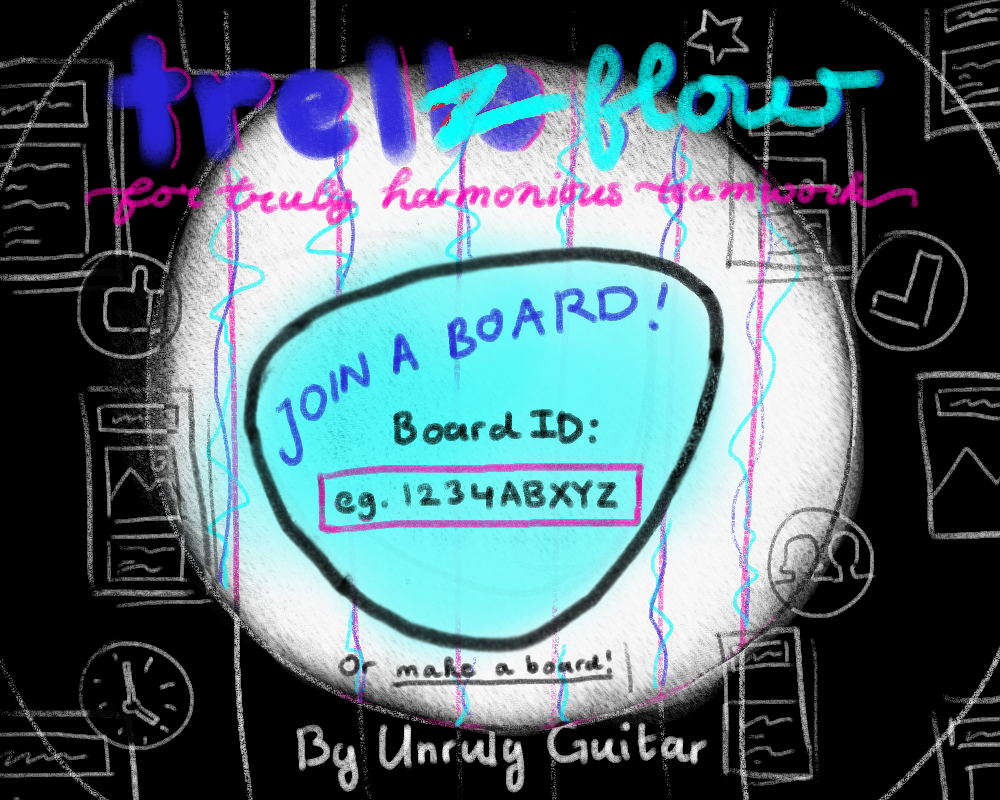
\includegraphics[width=11cm]{mock0}}
			\captionof{figure}{A mock of the join screen}
		\end{center}

		\begin{center}
			\shadowbox{
				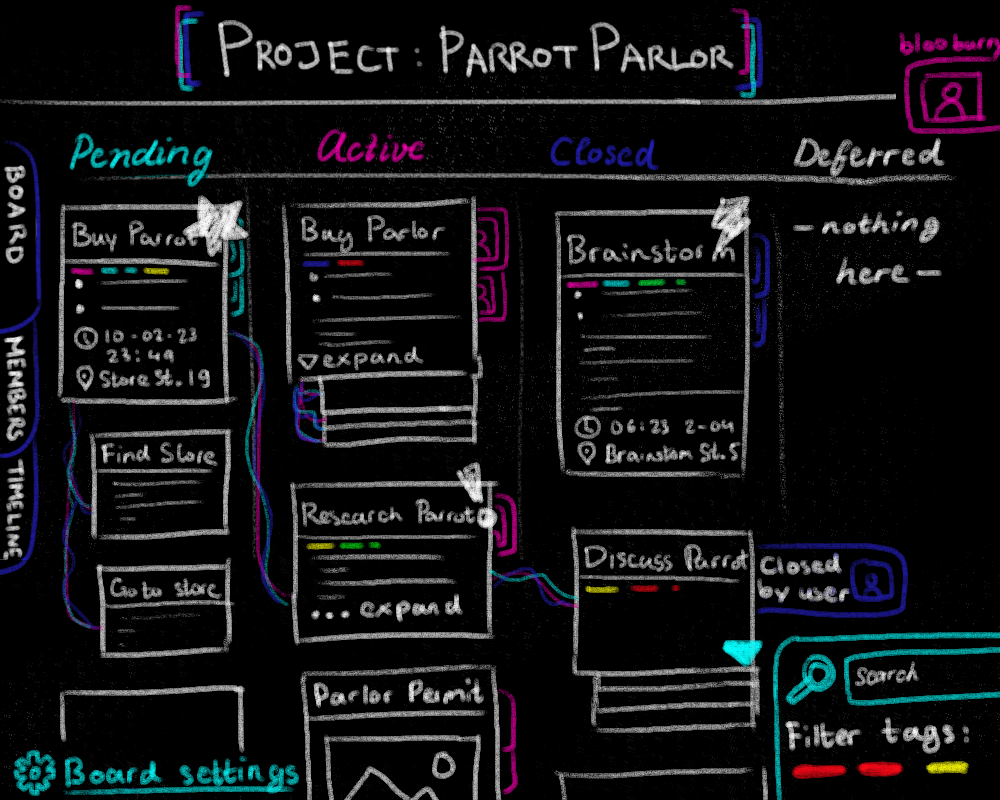
\includegraphics[width=11cm]{mock3}}
			\captionof{figure}{A mock of the board screen}
		\end{center}
		\begin{center}
			\shadowbox{
				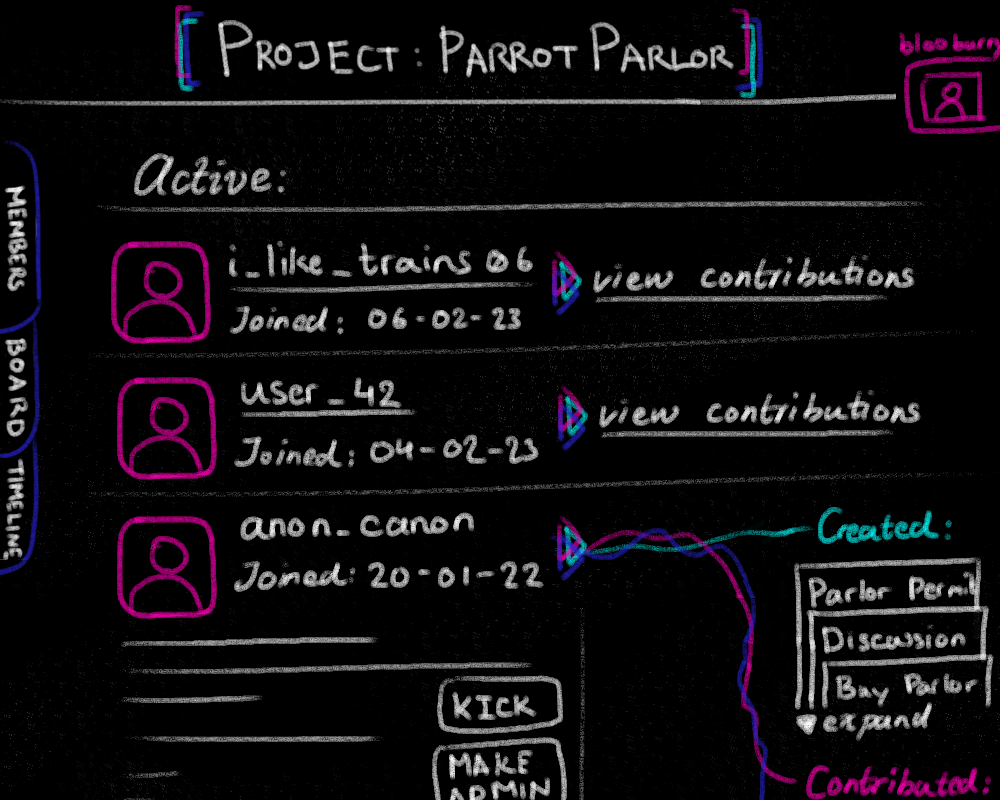
\includegraphics[width=11cm]{mock2}}
			\captionof{figure}{A mock of the analytics screen}
		\end{center}

	\begin{center}
		\shadowbox{
			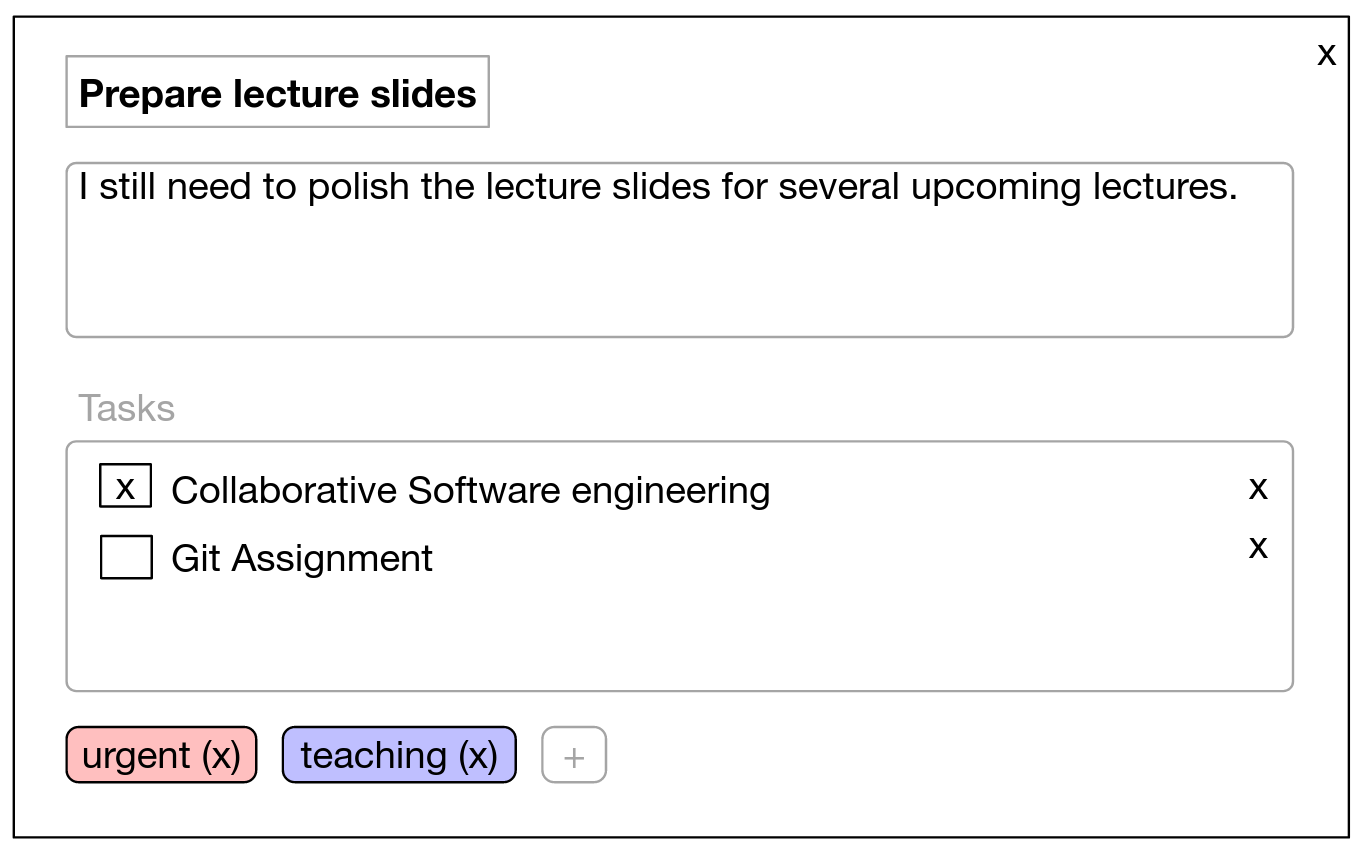
\includegraphics[width=10cm]{mock1}}
		\captionof{figure}{A mock of the loading screen}
	\end{center}


	\lfoot{\small \XeLaTeX \hspace{0.1cm} 3.14}

\end{document}
